% This must be in the first 5 lines to tell arXiv to use pdfLaTeX, which is strongly recommended.
\pdfoutput=1
% In particular, the hyperref package requires pdfLaTeX in order to break URLs across lines.

\documentclass[11pt]{article}

% Change "review" to "final" to generate the final (sometimes called camera-ready) version.
% Change to "preprint" to generate a non-anonymous version with page numbers.
\usepackage[final]{style/acl}

% Standard package includes
\usepackage{times}
\usepackage{latexsym}
\usepackage{longtable}
\usepackage{caption}
\usepackage{enumitem}
\usepackage{hyperref}




% For proper rendering and hyphenation of words containing Latin characters (including in bib files)
\usepackage[T1]{fontenc}
% For Vietnamese characters
% \usepackage[T5]{fontenc}
% See https://www.latex-project.org/help/documentation/encguide.pdf for other character sets

% This assumes your files are encoded as UTF8
\usepackage[utf8]{inputenc}

% This is not strictly necessary, and may be commented out,
% but it will improve the layout of the manuscript,
% and will typically save some space.
\usepackage{microtype}

% This is also not strictly necessary, and may be commented out.
% However, it will improve the aesthetics of text in
% the typewriter font.
\usepackage{inconsolata}

%Including images in your LaTeX document requires adding
%additional package(s)
\usepackage{graphicx}

% Custom Packages
\usepackage{amssymb}
\usepackage{amsmath}
\usepackage{subcaption}
\usepackage{booktabs}
\usepackage{xcolor}
\usepackage{multirow}
\usepackage{colortbl}
\usepackage{enumitem}

% support for Chinese
\usepackage{CJKutf8}

% If the title and author information does not fit in the area allocated, uncomment the following
%
%\setlength\titlebox{<dim>}
%
% and set <dim> to something 5cm or larger.

\title{Cognitive Alignment: Reducing Order Bias in MCQ Answering}
% Author information can be set in various styles:
% For several authors from the same institution:
\author{Eric Bennett\textsuperscript{2}, Su Bao\textsuperscript{1} \\
\textsuperscript{2}Dept. of Industrial Engineering, National Taiwan University \\ 
\textsuperscript{2}Dept. of Computer Science, University of Maryland, College Park \\ ebenne92@umd.edu, r13546027@ntu.edu.tw
}

% \author{Author 1 \and ... \and Author n \\
%         Address line \\ ... \\ Address line}
% if the names do not fit well on one line use
%         Author 1 \\ {\bf Author 2} \\ ... \\ {\bf Author n} \\
% For authors from different institutions:
% \author{Author 1 \\ Address line \\  ... \\ Address line
%         \And  ... \And
%         Author n \\ Address line \\ ... \\ Address line}
% To start a separate ``row'' of authors use \AND, as in
% \author{Author 1 \\ Address line \\  ... \\ Address line
%         \AND
%         Author 2 \\ Address line \\ ... \\ Address line \And
%         Author 3 \\ Address line \\ ... \\ Address line}

% ## Example by hyojung
% \author{HyoJung Han \\
% Computer Science\\
%   University of Maryland \\
%   \texttt{hjhan@cs.umd.edu} \\
%   \And
%   Kevin Duh \\
%   HLTCOE\\
%   Johns Hopkins University \\
%   \texttt{kevinduh@cs.jhu.edu} \\
%   \And
%   Marine Carpuat \\
% Computer Science\\
%   University of Maryland \\
%   \texttt{marine@cs.umd.edu} \\
%   }


%\author{
%  \textbf{First Author\textsuperscript{1}},
%  \textbf{Second Author\textsuperscript{1,2}},
%  \textbf{Third T. Author\textsuperscript{1}},
%  \textbf{Fourth Author\textsuperscript{1}},
%\\
%  \textbf{Fifth Author\textsuperscript{1,2}},
%  \textbf{Sixth Author\textsuperscript{1}},
%  \textbf{Seventh Author\textsuperscript{1}},
%  \textbf{Eighth Author \textsuperscript{1,2,3,4}},
%\\
%  \textbf{Ninth Author\textsuperscript{1}},
%  \textbf{Tenth Author\textsuperscript{1}},
%  \textbf{Eleventh E. Author\textsuperscript{1,2,3,4,5}},
%  \textbf{Twelfth Author\textsuperscript{1}},
%\\
%  \textbf{Thirteenth Author\textsuperscript{3}},
%  \textbf{Fourteenth F. Author\textsuperscript{2,4}},
%  \textbf{Fifteenth Author\textsuperscript{1}},
%  \textbf{Sixteenth Author\textsuperscript{1}},
%\\
%  \textbf{Seventeenth S. Author\textsuperscript{4,5}},
%  \textbf{Eighteenth Author\textsuperscript{3,4}},
%  \textbf{Nineteenth N. Author\textsuperscript{2,5}},
%  \textbf{Twentieth Author\textsuperscript{1}}
%\\
%\\
%  \textsuperscript{1}Affiliation 1,
%  \textsuperscript{2}Affiliation 2,
%  \textsuperscript{3}Affiliation 3,
%  \textsuperscript{4}Affiliation 4,
%  \textsuperscript{5}Affiliation 5
%\\
%  \small{
%    \textbf{Correspondence:} \href{mailto:email@domain}{email@domain}
%  }
%}


\begin{document}
\maketitle
%%%%%%%%%%%%%%%%%%%%%%%%%%%%%%%%%%%%%%%%%%%%%%%%%%%%%%%%%%%%%%%
%%  Abstract
%%%%%%%%%%%%%%%%%%%%%%%%%%%%%%%%%%%%%%%%%%%%%%%%%%%%%%%%%%%%%%%
\begin{abstract}
Large language models (LLMs) have achieved impressive performance on multiple-choice question answering tasks in zero-shot settings. However, recent studies reveal that LLM predictions can be sensitive to the order in which answer options are presented, a phenomenon known as \textit{order bias}. In this work, we conduct a systematic analysis of order bias in LLMs using a bilingual (English-Chinese) multiple-choice-question (MCQ) dataset spanning 17 knowledge domains. After removing inconsistent question pairs, we evaluate 1,700 aligned examples under various prompting strategies using GPT-4o and mistral-small. Our findings confirm that order bias affects model outputs, even when semantic content is held constant. We further propose a simple calibration method, Cognitive Alignment, that mitigates this bias across option permutations. This study highlights a critical limitation in current LLM evaluation paradigms and provides practical guidance for designing more robust prompting methods.
\end{abstract}
%%%%%%%%%%%%%%%%%%%%%%%%%%%%%%%%%%%%%%%%%%%%%%%%%%%%%%%%%%%%%%%
%%  Introduction
%%%%%%%%%%%%%%%%%%%%%%%%%%%%%%%%%%%%%%%%%%%%%%%%%%%%%%%%%%%%%%%
\section{Introduction}
\label{sec:intro}

Large Language Models (LLMs) have shown immense promise in solving multiple choice questions in a zero-shot fashion \citep{kojima2022large}. However, LLMs have also shown to exhibit biases across answer choice order. Order bias refers to the phenomenon in which a model's response is influenced not by the semantic content of each answer, but by its position in the list. 
Recent work by \citet{pezeshkpour2023optionorder} demonstrates that reordering options in multiple-choice questions can lead to substantial variation in accuracy—up to 75\% for GPT-4—indicating that current LLMs may not be as objective or consistent as expected, especially in zero- or few-shot evaluation settings.
To systematically evaluate order bias, we compile a bilingual MCQ dataset spanning 17 knowledge domains following the categorization of \citet{hendryckstest2021}. After removing inconsistent examples across languages, we obtain 1,700 English-Chinese aligned question pairs. We evaluate zero-shot prompting techniques using state-of-the-art LLMs including GPT-4o and mistral-small, comparin Chain-of-Thought(CoT) and Direct Prompting against our proposed novel method.

%%%%%%%%%%%%%%%%%%%%%%%%%%%%%%%%%%%%%%%%%%%%%%%%%%%%%%%%%%%%%%%
%%  Methods
%%%%%%%%%%%%%%%%%%%%%%%%%%%%%%%%%%%%%%%%%%%%%%%%%%%%%%%%%%%%%%%
\section{Test Set}
\label{sec:dataset}

For this experiment, we use both English and Chinese versions of the MMLU data set introduced in \citet{hendryckstest2021}. For Chinese, we use a translated version of the benchmark made available by OpenAI at \url{https://openaipublic.blob.core.windows.net/simple-evals/mmlu_ZH-CN.csv}. Throughout the cleaning process we preserve row alignment between the two languages to ensure identical questions are being considered.

\subsection{Data Cleaning}


A total of 176 rows of our bilingual dataset were found to have different correct answer values for the two languages, which were removed to reduce complexity.

We next divide the data set into subcategories following the structure in \citet{hendryckstest2021}. The subcategories are as follows: biology, business, chemistry, computer science, culture, economics, engineering, geography, health, history, law, math, other, philosophy, physics, politics, and psychology. From each subcategory, we sample 100 aligned English-Chinese question pairs, resulting in a total of 1,700 questions.

%%%%%%%%%%%%%%%%%%%%%%%%%%%%%%%%%%%%%%%%%%%%%%%%%%%%%%%%%%%%%%%
%%  Experiment Settings
%%%%%%%%%%%%%%%%%%%%%%%%%%%%%%%%%%%%%%%%%%%%%%%%%%%%%%%%%%%%%%%
\section{Methods}
\label{sec:method}

% \subsection{Baseline Methods}
To compare the results of our novel method, we used a number of baseline values, including both CoT and Direct Prompting. We use GPT-4o \citep{OpenAI2024-em} to show SoTA zero-shot Direct Prompting results, and mistral-small \citep{mistral_small_24b_2025} for Direct Prompting, CoT, and our novel method.

For each method, answers are generated for 4 permutations of each of the 1,700 questions. The questions are answered with the correct answer being located in A, B, C, and D positions. By contrasting the performance between permutations we generate the results shown in Section~\ref{sec:results}.

\subsection{Cognitive Alignment for MCQ Answering}

We present Cognitive Alignment(CA) as a method of fully removing order bias from the process of LLM MCQ answering. The process begins by using the LLM to answer the given question without any access to the provided choices. Next, both the LLM answer and the 4 possible answers are embedded using an embedding model. \footnote{In our experiment we use the distiluse-base-multilingual-cased-v2 (cite) embedding model because of its training in both English and Chinese.} Finally, the cosine similarity between the embedded LLM answer and the 4 answer choices is calculated, and the answer choice with the highest similarity is selected as the predicted answer.

\begin{equation}
\text{Answer} = \max_{i \in \{1, 2, 3, 4\}} \text{sim}(\text{LLM}, A_i)
\end{equation}


By never providing the answer choices to the LLM directly, order is fundamentally never considered. This inherently removes the ability for a given order to influence the LLM.

\paragraph{CA-Adjusted MCQ Answering}

While the pure CA approach completely removes the possibility of order bias, it has a major drawback- a large decrease in accuracy. Our results show pure CA on our English and Chinese datasets have an accuracy of 43\% and 38.333\% respectively, a drop from Direct Prompting of 38.044\% and 35\% (respectively). With such a major loss, we propose a second novel method, CA-Adjusted MCQ Answering, to balance the benefits of Direct Prompting accuracy and the reduction in order bias of CA.

CA-Adjusted MCQ Answering works by removing potential answer choices as selections based on what CA judges as "worse" answers. Given a set of similarity scores for A, B, C, D answer choices, any choice within a certain distance (cutoff value) from the highest similarity value are replaced with "DO NOT PICK THIS OPTION" in the dataset, reducing the distractions provided to the LLM when answering.

For example, consider the following:

\noindent\textbf{Question} \\
The soils of which of the following biomes has the highest rate of leaching and cycling of nutrients?

\vspace{0.5em}

\noindent\textbf{Answer choices}
\begin{enumerate}[label=\Alph*., itemsep=0pt, topsep=0pt]
    \item Tropical rain forest
    \item Tundra
    \item Taiga
    \item Desert
\end{enumerate}


\vspace{0.5em}

\noindent\textbf{Free-response answer generated by CA method:} \\
\textit{Tropical Rainforest}

\vspace{0.5em}

\noindent\textbf{Similarity scores generated by CA method}

\begin{center}
\begin{tabular}{@{}ll@{}}
\toprule
\textbf{Choice} & \textbf{Similarity Score} \\
\midrule
A & 0.96880 \\
B & 0.17935 \\
C & 0.19457 \\
D & 0.34539 \\
\bottomrule
\end{tabular}
\end{center}

\vspace{0.5em}

\noindent\textbf{New potential answer choices provided with a cutoff value of 0.459}
\begin{enumerate}[label=\Alph*., itemsep=0pt, topsep=0pt]
    \item Tropical rain forest
    \item DO NOT PICK THIS OPTION
    \item DO NOT PICK THIS OPTION
    \item DO NOT PICK THIS OPTION
\end{enumerate}


By removing low-confidence answers, the LLM is less likely to choose incorrect answers due to order bias, and by adjusting the cutoff value, we can balance the lower order bias of CA and the better accuracy of Direct Prompting.

We choose the cutoff value 0.459 in our testing as in every case where the difference between the highest and second highest similarity value is greater than or equal to 0.459 there is a 100\% accuracy (the correct answer is always chosen in the pure CA strategy in these cases).

% \subsection{Iterative Elimination for MCQ Answering}
% The first idea!
% do this if we have to do it like this!

%%%%%%%%%%%%%%%%%%%%%%%%%%%%%%%%%%%%%%%%%%%%%%%%%%%%%%%%%%%%%%%
%%  Results
%%%%%%%%%%%%%%%%%%%%%%%%%%%%%%%%%%%%%%%%%%%%%%%%%%%%%%%%%%%%%%%
\section{Results}
\label{sec:results}

\subsection{Metrics for Order Bias}
\label{sec:metrics}

To quantify the impact of answer permutation on model predictions, we adopt three metrics widely used in recent work: \textbf{Relative Standard Deviation (RSD)} \citep{reif-schwartz-2024-beyond}, \textbf{Recall Standard Deviation (RStd)} \citep{zheng2024largelanguagemodelsrobust}, and \textbf{Fluctuation Rate (FR)} \citep{wei-etal-2024-unveiling}.  
Each captures a different facet of instability under order variation.

\paragraph{Relative Standard Deviation (RSD).}
RSD measures the sensitivity of overall accuracy to answer permutations.  
Let $\{A_1,A_2,\dots,A_n\}$ denote the model’s accuracy under $n$ distinct answer orders. Then
\begin{align}
  \mathrm{RSD} &=
  \frac{\sqrt{\frac{1}{n}\sum_{i=1}^{n}(A_i-\overline{A})^2}}
       {\overline{A}}, \\
  \overline{A} &= \frac{1}{n}\sum_{i=1}^{n}A_i .
  \label{eq:rsd}
\end{align}
Higher values indicate greater variability in model-level performance across permutations.

\paragraph{Recall Standard Deviation (RStd).}
RStd captures how individual questions are affected by order shifts.  
For each question $q$, let $\{r_{q,1},\dots,r_{q,k}\}$ be the binary correctness across $k$ permutations. Then
\begin{align}
  \mathrm{RStd} &=
  \frac{1}{N}\sum_{q=1}^{N}
  \frac{
    \sqrt{\frac{1}{k}\sum_{j=1}^{k}(r_{q,j}-\overline{r_q})^2}
  }{
    \overline{r_q}+\varepsilon
  }, \\
  \overline{r_q} &= \frac{1}{k}\sum_{j=1}^{k}r_{q,j}.
  \label{eq:rstd}
\end{align}
Here $\varepsilon$ is a small constant to prevent division by zero. A larger RStd signals greater sample-level prediction instability.

\paragraph{Fluctuation Rate (FR).}
FR quantifies how often the predicted answer changes when the option order is permuted.  
Let $f_q$ be the number of unique predictions for question $q$ across the $k$ permutations:
\begin{equation}
  \mathrm{FR}=
  \frac{1}{N}\sum_{q=1}^{N}\frac{f_q-1}{k-1}.
  \label{eq:fr}
\end{equation}
FR ranges from $0$ (fully stable) to $1$ (changes prediction in every permutation), directly reflecting positional sensitivity.

\subsection{Overall Results}

The overall performance of each method across English and Chinese datasets are summarized in Table~\ref{tab:order_bias_results}, and Figure~\ref{fig:overall_results} visualizes the results of each method across metrics. Our proposed CA-adjusted MCQ Answering method (specifically with cutoff value 0.2) consistently reduced order bias compared to both Direct Prompting and CoT prompting across all evaluated metrics, only being beaten in RSD by the SoTA Direct Prompting method.

\begin{figure}[t]
    \centering
    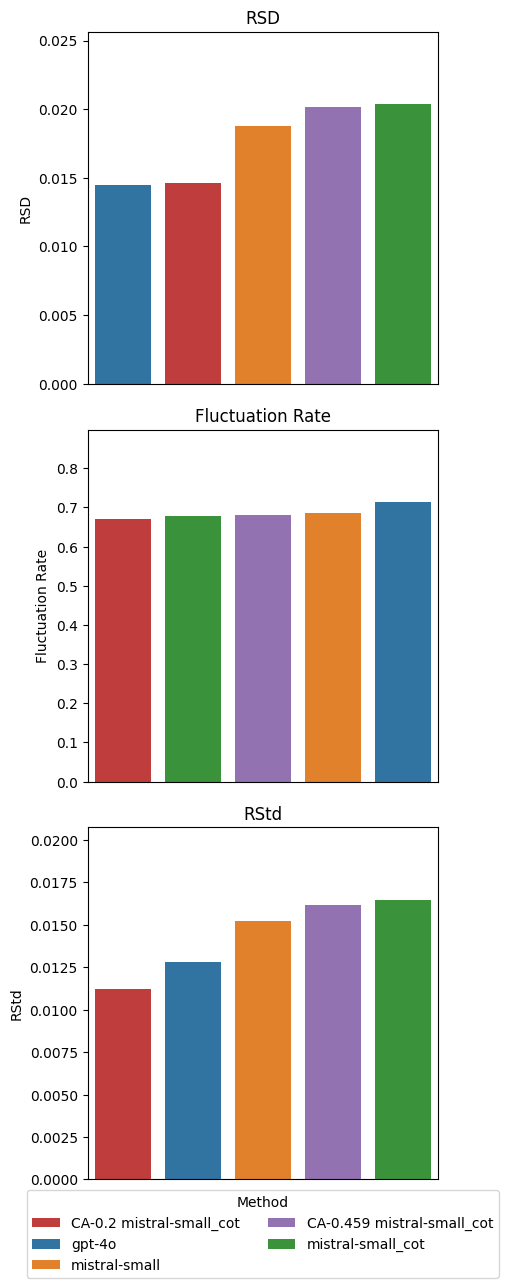
\includegraphics[height=0.63\textheight]{figures/overall.png}
    \caption{Comparison of the five methods on RSD, RStd, and Fluctuation Rate. Lower values indicate reduced order bias and improved stability.}
    \label{fig:overall_results}
\end{figure}

\begin{table*}[t]
\centering
\resizebox{\textwidth}{!}{
\begin{tabular}{l|cc|cc|cc|cc|}
\cline{2-9}
 & \multicolumn{2}{c|}{\textbf{Overall Accuracy}} & \multicolumn{2}{c|}{\textbf{RSD}} & \multicolumn{2}{c|}{\textbf{RStd}} & \multicolumn{2}{c|}{\textbf{Fluctuation Rate}} \\
\hline
\multicolumn{1}{|l|}{\textbf{Method}} & \textbf{English} & \textbf{Chinese} & \textbf{English} & \textbf{Chinese} & \textbf{English} & \textbf{Chinese} & \textbf{English} & \textbf{Chinese} \\
\hline
\multicolumn{1}{|l|}{\textbf{gpt-4o}} & \textbf{0.882794} & \textbf{0.849265} & \textbf{0.014487} & \textbf{0.019291} & 0.012789 & \textbf{0.016383} & 0.713088 & 0.701176 \\
\multicolumn{1}{|l|}{\textbf{mistral-small}} & 0.810441 & 0.733333 & 0.018762 & 0.032797 & 0.015205 & 0.024051 & 0.686029 & 0.658500 \\
\multicolumn{1}{|l|}{\textbf{mistral-small\_cot}} & 0.809412 & 0.748676 & 0.020342 & 0.044451 & 0.016465 & 0.033279 & 0.679265 & 0.660735 \\
\multicolumn{1}{|l|}{\textbf{CA-0.2 mistral-small\_cot}} & 0.766618 & 0.698235 & 0.014643 & 0.032861 & \textbf{0.011226} & 0.022945 & \textbf{0.671176} & \textbf{0.654412} \\
\multicolumn{1}{|l|}{\textbf{CA-0.459 mistral-small\_cot}} & 0.804118 & 0.743824 & 0.020140 & 0.042449 & 0.016195 & 0.031575 & 0.679559 & 0.660147 \\
\hline
\end{tabular}}
\caption{Evaluation of models across English and Mandarin on Overall Accuracy, Relative Standard Deviation (RSD), Recall Standard Deviation (RStd), and Fluctuation Rate (FR). For RSD, RStd, and FR lower scores indicate less order bias}
\label{tab:order_bias_results}
\end{table*}




\subsection{Order Sensitivity Across Languages}

We conducted our experiment with both English and Chinese to compare the order bias between the two languages. RSD, RStd, and Fluctuation Rate all varied by language across methods (see Figure~\ref{fig:language_results}), with RSD and RStd being consistently higher in Chinese than English, and Fluctuation Rate consistently being slightly lower.

Observing RSD and RStd across methods, our SoTA Direct Prompting method exceeds our CA-Adjusted method. This is likely a result of better multilingual capabilities in our SoTA GPT-4o model as opposed to mistral-small. The full results across languages can be found in Table~\ref{tab:order_bias_results}

\begin{figure*}[t]
    \centering
    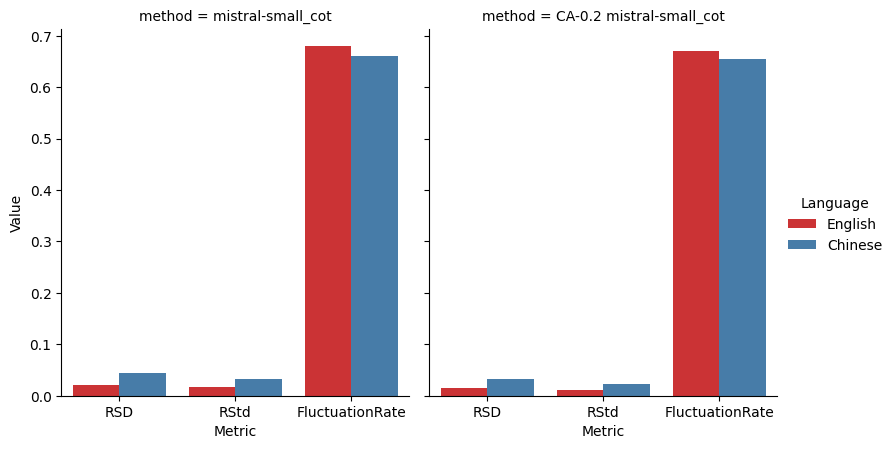
\includegraphics[width=\textwidth]{figures/language.png}
    \caption{Comparison of English vs. Mandarin for RSD, RStd, and Fluctuation Rate across \texttt{mistral-small\_cot} and \texttt{CA-0.2 mistral-small\_cot} methods. Lower RSD, RStd, or Fluctuation Rate values indicate reduced order bias}
    \label{fig:language_results}
\end{figure*}

\subsection{Order Sensitivity Across Subcategories}

To observe order bias in different knowledge domains, we contrast our metrics across the 17 subcategories defined in \citet{hendryckstest2021}, comparing SoTA Direct Prompting, CoT, and CA-adjusted CoT (with cutoff value 0.2 results). Figure~\ref{fig:subcategory_rsd} illustrates the English RSD values by subcategory for \texttt{mistral-small\_cot} versus \texttt{CA-0.2 mistral-small\_cot}.

Across these subcategories, the CA-Adjusted MCQ Answering method achieved lower values on a majority of metrics, improving order bias in 14 out of 17 cases. The subcategories in which CA-adjustment did not improve order bias include computer science, economics, and psychology. The full results across subcategories are found in Table~\ref{tab:order_bias_results}


\begin{figure*}[t]
    \centering
    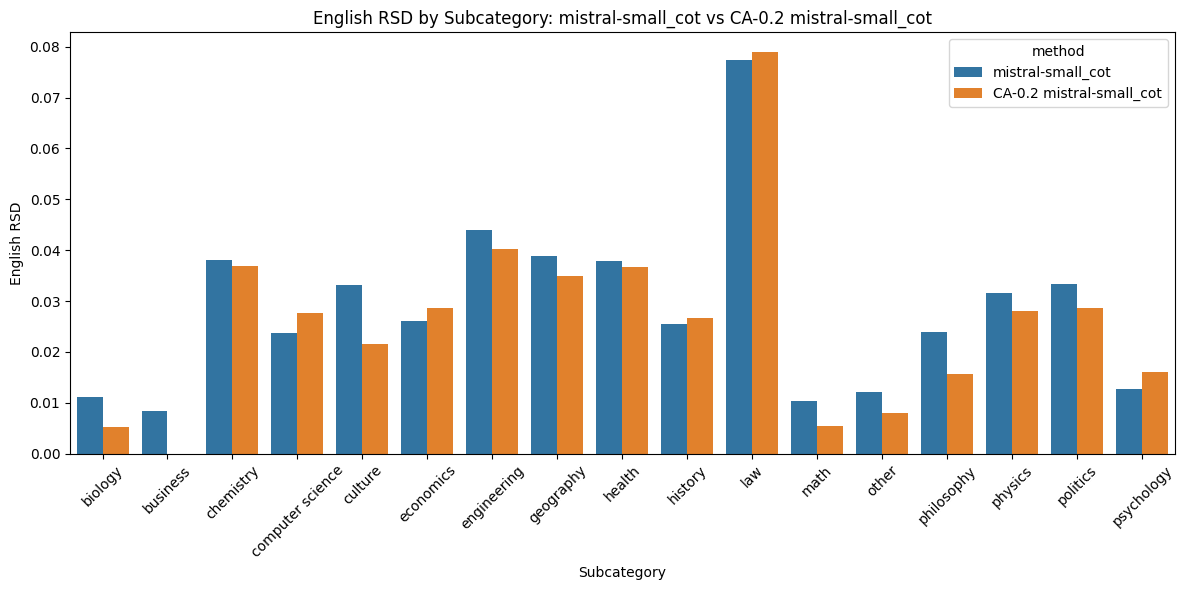
\includegraphics[width=\textwidth]{figures/subcategory.png}
    \caption{English RSD by Subcategory comparing \texttt{mistral-small\_cot} (blue) vs. \texttt{CA-0.2 mistral-small\_cot} (orange). Orange bars higher than blue indicate subcategories in which CA-Adjustment reduced order bias.}
    \label{fig:subcategory_rsd}
\end{figure*}


\subsection{Confidence vs. Order Bias}

Our CA-Adjusted method allows us to control the balance between order-bias reduction and accuracy by adjusting the cutoff value. A higher cutoff value results in less answer choices being removed, retaining accuracy but having little to no effect on order bias. A lower cutoff value removes more answer choices, lowering order bias more, but decreases accuracy as the chances of the correct answer being accidentally removed rise.

In our experiment, CA-Adjusted with cutoff value 0.2 clearly outperformed 0.459 in all recorded metrics as shown in Figure~\ref{fig:overall_results}, while cutoff value 0.459 was outperformed by Direct Prompting in both RStd and Fluctuation Rate. That being said, Table~\ref{tab:accuracy_results} shows the decreased accuracy of a cutoff value of 0.459 as opposed to 0.2. CA-Adjusted with a 0.459 cutoff value performs 5.04\% and 7.09\% better than with 0.2 in English and Chinese respectively.

Although the results of this test specifically compared the two cutoff values of 0.2 and 0.459, future research might benefit from exploring the impacts of further tuning of the cutoff value, as well as alternate ways of determining extraneous answer choices based on similarity scores.

\subsection{Takeaways from Cognitive Alignment} %maybe change the name
\label{sec:takeaways}

Cognitive Alignment and CA-Adjusted MCQ Answering both were successful in lowering order bias across knowledge domains and languages.

However, we also found a number of obvious drawbacks of the CA approach. For example, in the following question/answer pair we see a complete failure based on the format of the question:

\noindent\textbf{Question} \\
What was 'democratic enlargement'?

\vspace{0.5em}

\noindent\textbf{Answer choices}
\begin{enumerate}[label=\Alph*., itemsep=0pt, topsep=0pt]
    \item A proposal for reform of the US system of government
    \item A proposal for the extension of democratic rule globally
    \item A proposal for the extension of free markets
    \item Both b and c
\end{enumerate}


\vspace{0.5em}

\noindent\textbf{Free-response answer generated by CA method:} \\
\textit{Democratic enlargement refers to the process of expanding democratic governance and institutions, often within a region or globally. It involves promoting democracy in countries that are transitioning from authoritarian regimes or have limited democratic practices. This can include efforts such as supporting free elections, strengthening civil society, and fostering human rights.}

\vspace{0.5em}

\noindent\textbf{Similarity scores generated by CA method}

\begin{center}
\begin{tabular}{@{}ll@{}}
\toprule
\textbf{Choice} & \textbf{Similarity Score} \\
\midrule
A & 0.1847597062587738 \\
B & 0.517923891544342 \\
C & 0.19801126420497894 \\
D & -0.06396911293268204 \\
\bottomrule
\end{tabular}
\end{center}

While "Both b and c" is the correct answer, the alignment method cannot detect the similarity between it and the free response answer because the answer choice merely references other answer choices. 

Overall, it is clear that this method produces a tradeoff between accuracy and reduced order bias. Our most successful method at reducing order bias, CA-0.2 mistral-small\_cot, led to a 5.49\% and 7.57\% accuracy decrease in English and Chinese respectively. A full comparison of accuracy across CA methods is located in Table~\ref{tab:accuracy_results}.



\begin{table}[h]
\centering
\small
\begin{tabular}{|l|c|c|}
\hline
\textbf{Method} & \textbf{English} & \textbf{Chinese} \\
\hline
Pure CA & 0.43000 & 0.38353 \\
CA-0.2 mistral-small\_cot & 0.77059 & 0.69706 \\
CA-0.459 mistral-small\_cot & 0.80941 & 0.74647 \\
mistral-small\_cot & 0.81529 & 0.75412 \\
\hline
\end{tabular}
\caption{Accuracy of each method on English and Chinese.}
\label{tab:accuracy_results}
\end{table}


\subsection{Future Research Paths} %maybe don't make a subsection
While the lackluster accuracy performance of the pure CA method would suggest it shouldn't be used in multiple choice answering as is, the inherent, complete removal of order bias suggests incorporating alignment might still be useful in reducing order bias. 

The CA-Adjusted method provides an example of how this could be done, but falls short of a widely implementable method. Future research might refine the method of deciding on specific answer choices to remove to avoid issues like those shown in~\ref{sec:takeaways}, or use other methods of removing problematic answer choices before being feeding the ordered questions to an LLM.

The code and experimental framework used in this paper are available at: \url{https://github.com/softly-undefined/NLP_final}.


%%%%%%%%%%%%%%%%%%%%%%%%%%%%%%%%%%%%%%%%%%%%%%%%%%%%%%%%%%%%%%%
%%  Related Work
%%%%%%%%%%%%%%%%%%%%%%%%%%%%%%%%%%%%%%%%%%%%%%%%%%%%%%%%%%%%%%%
% \input{sections/50-related-works}

%%%%%%%%%%%%%%%%%%%%%%%%%%%%%%%%%%%%%%%%%%%%%%%%%%%%%%%%%%%%%%%%%
%%  Any Final Conclusions
%%%%%%%%%%%%%%%%%%%%%%%%%%%%%%%%%%%%%%%%%%%%%%%%%%%%%%%%%%%%%%%%%
%\section{Conclusion and Future Work}
\label{sec:conclusion}


%%%%%%%%%%%%%%%%%%%%%%%%%%%%%%%%%%%%%%%%%%%%%%%%%%%%%%%%%%%%%%%%%
%%  Limitations & Ethics Statements 
%%%%%%%%%%%%%%%%%%%%%%%%%%%%%%%%%%%%%%%%%%%%%%%%%%%%%%%%%%%%%%%%%
% \section*{Acknowledgments}
need?

%%%%%%%%%%%%%%%%%%%%%%%%%%%%%%%%%%%%%%%%%%%%%%%%%%%%%%%%%%%%%%%%%
%%  Bibliography
%%%%%%%%%%%%%%%%%%%%%%%%%%%%%%%%%%%%%%%%%%%%%%%%%%%%%%%%%%%%%%%%%
\bibliography{bib/anthology, bib/custom}
%%%%%%%%%%%%%%%%%%%%%%%%%%%%%%%%%%%%%%%%%%%%%%%%%%%%%%%%%%%%%%%%%
%%  Appendices
%%%%%%%%%%%%%%%%%%%%%%%%%%%%%%%%%%%%%%%%%%%%%%%%%%%%%%%%%%%%%%%%%
\clearpage
\appendix
\setlength{\tabcolsep}{4pt}
{\footnotesize
\begin{longtable}{|l|cc|cc|cc|cc|}
\caption{Evaluation of models across English and Mandarin on Overall Accuracy, Relative Standard Deviation (RSD), Recall Standard Deviation (RStd), and Fluctuation Rate (FR). For RSD, RStd, and FR lower scores indicate better stability and less sensitivity to answer order permutations.}
\label{tab:order_bias_results}
\hline
 & \multicolumn{2}{c|}{\textbf{Overall Accuracy}} & \multicolumn{2}{c|}{\textbf{RSD}} & \multicolumn{2}{c|}{\textbf{RStd}} & \multicolumn{2}{c|}{\textbf{Fluctuation Rate}} \\
\hline
\multicolumn{1}{|l|}{\textbf{Method}} & \textbf{English} & \textbf{Chinese} & \textbf{English} & \textbf{Chinese} & \textbf{English} & \textbf{Chinese} & \textbf{English} & \textbf{Chinese} \\
\hline
\endfirsthead
\hline
 & \multicolumn{2}{c|}{\textbf{Overall Accuracy}} & \multicolumn{2}{c|}{\textbf{RSD}} & \multicolumn{2}{c|}{\textbf{RStd}} & \multicolumn{2}{c|}{\textbf{Fluctuation Rate}} \\
\hline
\multicolumn{1}{|l|}{\textbf{Method}} & \textbf{English} & \textbf{Chinese} & \textbf{English} & \textbf{Chinese} & \textbf{English} & \textbf{Chinese} & \textbf{English} & \textbf{Chinese} \\
\hline
\endlastfoot
\multicolumn{9}{|c|}{\textbf{Biology}} \\
\hline
\multicolumn{1}{|l|}{\textbf{gpt-4o}} & \textbf{0.920000} & \textbf{0.910000} & 0.015370 & \textbf{0.020560} & 0.014140 & \textbf{0.018710} & \textbf{0.707500} & 0.710000 \\
\multicolumn{1}{|l|}{\textbf{mistral-small\_cot}} & 0.900000 & 0.872500 & 0.011110 & 0.023450 & 0.010000 & 0.020460 & 0.712500 & 0.685000 \\
\multicolumn{1}{|l|}{\textbf{CA-0.2 mistral-small\_cot}} & 0.837500 & 0.772500 & \textbf{0.005170} & 0.043300 & \textbf{0.004330} & 0.033450 & \textbf{0.707500} & \textbf{0.667500} \\
\hline
\multicolumn{9}{|c|}{\textbf{Business}} \\
\hline
\multicolumn{1}{|l|}{\textbf{gpt-4o}} & \textbf{0.837500} & \textbf{0.875000} & 0.017660 & \textbf{0.020600} & 0.014790 & 0.018030 & \textbf{0.677500} & 0.700000 \\
\multicolumn{1}{|l|}{\textbf{mistral-small\_cot}} & 0.850000 & 0.790000 & 0.008320 & 0.042930 & 0.007070 & 0.033910 & 0.682500 & \textbf{0.670000} \\
\multicolumn{1}{|l|}{\textbf{CA-0.2 mistral-small\_cot}} & 0.840000 & 0.762500 & \textbf{0.000000} & 0.023410 & \textbf{0.000000} & \textbf{0.017850} & 0.690000 & 0.672500 \\
\hline
\multicolumn{9}{|c|}{\textbf{Chemistry}} \\
\hline
\multicolumn{1}{|l|}{\textbf{gpt-4o}} & \textbf{0.825000} & \textbf{0.830000} & \textbf{0.018180} & \textbf{0.014760} & \textbf{0.015000} & \textbf{0.012250} & 0.710000 & 0.705000 \\
\multicolumn{1}{|l|}{\textbf{mistral-small\_cot}} & 0.720000 & 0.700000 & 0.038040 & 0.039120 & 0.027390 & 0.027390 & 0.672500 & 0.662500 \\
\multicolumn{1}{|l|}{\textbf{CA-0.2 mistral-small\_cot}} & 0.647500 & 0.662500 & 0.036830 & 0.028990 & 0.023850 & 0.019200 & \textbf{0.660000} & \textbf{0.657500} \\
\hline
\multicolumn{9}{|c|}{\textbf{Computer science}} \\
\hline
\multicolumn{1}{|l|}{\textbf{gpt-4o}} & \textbf{0.882500} & \textbf{0.885000} & \textbf{0.016760} & 0.025890 & \textbf{0.014790} & 0.022910 & 0.712500 & 0.725000 \\
\multicolumn{1}{|l|}{\textbf{mistral-small\_cot}} & 0.790000 & 0.740000 & 0.023680 & 0.039400 & 0.018710 & 0.029150 & 0.672500 & \textbf{0.667500} \\
\multicolumn{1}{|l|}{\textbf{CA-0.2 mistral-small\_cot}} & 0.770000 & 0.727500 & 0.027550 & \textbf{0.024540} & 0.021210 & \textbf{0.017850} & \textbf{0.662500} & 0.677500 \\
\hline
\multicolumn{9}{|c|}{\textbf{Culture}} \\
\hline
\multicolumn{1}{|l|}{\textbf{gpt-4o}} & 0.847500 & \textbf{0.915000} & \textbf{0.009780} & \textbf{0.039020} & \textbf{0.008290} & 0.035710 & 0.717500 & 0.702500 \\
\multicolumn{1}{|l|}{\textbf{mistral-small\_cot}} & \textbf{0.862500} & 0.810000 & 0.033180 & 0.057240 & 0.028610 & 0.046370 & 0.702500 & 0.687500 \\
\multicolumn{1}{|l|}{\textbf{CA-0.2 mistral-small\_cot}} & 0.827500 & 0.700000 & 0.021580 & 0.050510 & 0.017850 & \textbf{0.035360} & \textbf{0.692500} & \textbf{0.670000} \\
\hline
\multicolumn{9}{|c|}{\textbf{Economics}} \\
\hline
\multicolumn{1}{|l|}{\textbf{gpt-4o}} & \textbf{0.872500} & \textbf{0.907500} & 0.029640 & 0.032480 & 0.025860 & 0.029470 & 0.712500 & 0.720000 \\
\multicolumn{1}{|l|}{\textbf{mistral-small\_cot}} & 0.832500 & 0.742500 & \textbf{0.026010} & \textbf{0.025860} & \textbf{0.021650} & \textbf{0.019200} & 0.707500 & 0.695000 \\
\multicolumn{1}{|l|}{\textbf{CA-0.2 mistral-small\_cot}} & 0.780000 & 0.732500 & 0.028670 & 0.031090 & 0.022360 & 0.022780 & \textbf{0.682500} & \textbf{0.692500} \\
\hline
\multicolumn{9}{|c|}{\textbf{Engineering}} \\
\hline
\multicolumn{1}{|l|}{\textbf{gpt-4o}} & \textbf{0.785000} & \textbf{0.827500} & 0.052910 & 0.053620 & 0.041530 & 0.044370 & 0.667500 & 0.695000 \\
\multicolumn{1}{|l|}{\textbf{mistral-small\_cot}} & 0.762500 & 0.687500 & 0.043870 & 0.086280 & 0.033450 & 0.059320 & 0.650000 & 0.640000 \\
\multicolumn{1}{|l|}{\textbf{CA-0.2 mistral-small\_cot}} & 0.680000 & 0.622500 & \textbf{0.040270} & \textbf{0.048690} & \textbf{0.027390} & \textbf{0.030310} & \textbf{0.625000} & \textbf{0.635000} \\
\hline
\multicolumn{9}{|c|}{\textbf{Health}} \\
\hline
\multicolumn{1}{|l|}{\textbf{gpt-4o}} & \textbf{0.807500} & \textbf{0.815000} & 0.045820 & \textbf{0.020350} & 0.037000 & \textbf{0.016580} & 0.687500 & 0.695000 \\
\multicolumn{1}{|l|}{\textbf{mistral-small\_cot}} & 0.770000 & 0.740000 & 0.037860 & 0.054890 & 0.029150 & 0.040620 & 0.652500 & 0.625000 \\
\multicolumn{1}{|l|}{\textbf{CA-0.2 mistral-small\_cot}} & 0.735000 & 0.667500 & \textbf{0.036630} & 0.061200 & \textbf{0.026930} & 0.040850 & \textbf{0.650000} & \textbf{0.602500} \\
\hline
\multicolumn{9}{|c|}{\textbf{History}} \\
\hline
\multicolumn{1}{|l|}{\textbf{gpt-4o}} & \textbf{0.885000} & \textbf{0.920000} & \textbf{0.024630} & \textbf{0.007690} & 0.021790 & \textbf{0.007070} & 0.717500 & 0.725000 \\
\multicolumn{1}{|l|}{\textbf{mistral-small\_cot}} & 0.830000 & 0.770000 & 0.025560 & 0.042080 & 0.021210 & 0.032400 & 0.707500 & \textbf{0.680000} \\
\multicolumn{1}{|l|}{\textbf{CA-0.2 mistral-small\_cot}} & 0.775000 & 0.735000 & 0.026600 & 0.020410 & \textbf{0.020620} & 0.015000 & \textbf{0.697500} & 0.697500 \\
\hline
\multicolumn{9}{|c|}{\textbf{Geography}} \\
\hline
\multicolumn{1}{|l|}{\textbf{gpt-4o}} & \textbf{0.882500} & \textbf{0.907500} & 0.040360 & \textbf{0.004770} & 0.035620 & \textbf{0.004330} & 0.702500 & 0.732500 \\
\multicolumn{1}{|l|}{\textbf{mistral-small\_cot}} & 0.842500 & 0.772500 & 0.038800 & 0.055960 & 0.032690 & 0.043230 & \textbf{0.690000} & 0.677500 \\
\multicolumn{1}{|l|}{\textbf{CA-0.2 mistral-small\_cot}} & 0.842500 & 0.725000 & \textbf{0.034980} & 0.062830 & \textbf{0.029470} & 0.045550 & 0.695000 & \textbf{0.657500} \\
\hline
\multicolumn{9}{|c|}{\textbf{Law}} \\
\hline
\multicolumn{1}{|l|}{\textbf{gpt-4o}} & \textbf{0.675000} & \textbf{0.747500} & \textbf{0.055920} & \textbf{0.043730} & \textbf{0.037750} & \textbf{0.032690} & 0.667500 & 0.670000 \\
\multicolumn{1}{|l|}{\textbf{mistral-small\_cot}} & 0.622500 & 0.520000 & 0.077350 & 0.129720 & 0.048150 & 0.067450 & 0.625000 & 0.620000 \\
\multicolumn{1}{|l|}{\textbf{CA-0.2 mistral-small\_cot}} & 0.562500 & 0.417500 & 0.078880 & 0.099300 & 0.044370 & 0.041460 & \textbf{0.610000} & \textbf{0.592500} \\
\hline
\multicolumn{9}{|c|}{\textbf{Math}} \\
\hline
\multicolumn{1}{|l|}{\textbf{gpt-4o}} & \textbf{0.917500} & \textbf{0.927500} & 0.009040 & \textbf{0.008940} & 0.008290 & \textbf{0.008290} & 0.722500 & 0.727500 \\
\multicolumn{1}{|l|}{\textbf{mistral-small\_cot}} & 0.802500 & 0.775000 & 0.010330 & 0.049560 & 0.008290 & 0.038410 & \textbf{0.645000} & 0.630000 \\
\multicolumn{1}{|l|}{\textbf{CA-0.2 mistral-small\_cot}} & 0.792500 & 0.775000 & \textbf{0.005460} & 0.042310 & \textbf{0.004330} & 0.032790 & \textbf{0.645000} & \textbf{0.627500} \\
\hline
\multicolumn{9}{|c|}{\textbf{Philosophy}} \\
\hline
\multicolumn{1}{|l|}{\textbf{gpt-4o}} & \textbf{0.807500} & \textbf{0.847500} & 0.022110 & \textbf{0.021070} & 0.017850 & \textbf{0.017850} & 0.700000 & 0.715000 \\
\multicolumn{1}{|l|}{\textbf{mistral-small\_cot}} & 0.755000 & 0.665000 & 0.023880 & 0.093610 & 0.018030 & 0.062250 & \textbf{0.652500} & \textbf{0.595000} \\
\multicolumn{1}{|l|}{\textbf{CA-0.2 mistral-small\_cot}} & 0.715000 & 0.622500 & \textbf{0.015640} & 0.090430 & \textbf{0.011180} & 0.056290 & \textbf{0.652500} & \textbf{0.595000} \\
\hline
\multicolumn{9}{|c|}{\textbf{Physics}} \\
\hline
\multicolumn{1}{|l|}{\textbf{gpt-4o}} & \textbf{0.910000} & \textbf{0.932500} & \textbf{0.015540} & \textbf{0.019150} & \textbf{0.014140} & \textbf{0.017850} & 0.722500 & 0.730000 \\
\multicolumn{1}{|l|}{\textbf{mistral-small\_cot}} & 0.817500 & 0.760000 & 0.031630 & 0.026320 & 0.025860 & 0.020000 & 0.672500 & 0.667500 \\
\multicolumn{1}{|l|}{\textbf{CA-0.2 mistral-small\_cot}} & 0.732500 & 0.687500 & 0.027940 & 0.027930 & 0.020460 & 0.019200 & \textbf{0.655000} & \textbf{0.662500} \\
\hline
\multicolumn{9}{|c|}{\textbf{Politics}} \\
\hline
\multicolumn{1}{|l|}{\textbf{gpt-4o}} & \textbf{0.820000} & \textbf{0.867500} & 0.039520 & 0.022140 & 0.032400 & 0.019200 & 0.692500 & 0.710000 \\
\multicolumn{1}{|l|}{\textbf{mistral-small\_cot}} & 0.820000 & 0.750000 & 0.033400 & 0.049890 & 0.027390 & 0.037420 & 0.685000 & 0.655000 \\
\multicolumn{1}{|l|}{\textbf{CA-0.2 mistral-small\_cot}} & 0.797500 & 0.690000 & \textbf{0.028560} & \textbf{0.017750} & \textbf{0.022780} & \textbf{0.012250} & \textbf{0.682500} & \textbf{0.647500} \\
\hline
\multicolumn{9}{|c|}{\textbf{Psychology}} \\
\hline
\multicolumn{1}{|l|}{\textbf{gpt-4o}} & \textbf{0.875000} & \textbf{0.952500} & 0.018950 & \textbf{0.013640} & 0.016580 & \textbf{0.012990} & 0.700000 & 0.735000 \\
\multicolumn{1}{|l|}{\textbf{mistral-small\_cot}} & \textbf{0.875000} & 0.820000 & \textbf{0.012780} & 0.028600 & \textbf{0.011180} & 0.023450 & 0.702500 & \textbf{0.687500} \\
\multicolumn{1}{|l|}{\textbf{CA-0.2 mistral-small\_cot}} & 0.807500 & 0.785000 & 0.016090 & 0.026260 & 0.012990 & 0.020620 & \textbf{0.687500} & \textbf{0.687500} \\
\hline
\multicolumn{9}{|c|}{\textbf{Other}} \\
\hline
\multicolumn{1}{|l|}{\textbf{gpt-4o}} & 0.887500 & \textbf{0.940000} & 0.012280 & \textbf{0.007520} & 0.010900 & \textbf{0.007070} & \textbf{0.702500} & 0.725000 \\
\multicolumn{1}{|l|}{\textbf{mistral-small\_cot}} & \textbf{0.907500} & 0.812500 & 0.012010 & 0.040240 & 0.010900 & 0.032690 & 0.715000 & 0.687500 \\
\multicolumn{1}{|l|}{\textbf{CA-0.2 mistral-small\_cot}} & 0.890000 & 0.785000 & \textbf{0.007950} & 0.051350 & \textbf{0.007070} & 0.040310 & 0.715000 & \textbf{0.682500} \\
\hline
\end{longtable}
}


\end{document}

\begin{document}
\maketitle
\begin{abstract}
This document is a supplement to the general instructions for *ACL authors. It contains instructions for using the \LaTeX{} style files for ACL conferences.
The document itself conforms to its own specifications, and is therefore an example of what your manuscript should look like.
These instructions should be used both for papers submitted for review and for final versions of accepted papers.
\end{abstract}

\section{Introduction}

These instructions are for authors submitting papers to *ACL conferences using \LaTeX. They are not self-contained. All authors must follow the general instructions for *ACL proceedings,\footnote{\url{http://acl-org.github.io/ACLPUB/formatting.html}} and this document contains additional instructions for the \LaTeX{} style files.

The templates include the \LaTeX{} source of this document (\texttt{acl\_latex.tex}),
the \LaTeX{} style file used to format it (\texttt{acl.sty}),
an ACL bibliography style (\texttt{acl\_natbib.bst}),
an example bibliography (\texttt{custom.bib}),
and the bibliography for the ACL Anthology (\texttt{anthology.bib}).

\section{Engines}

To produce a PDF file, pdf\LaTeX{} is strongly recommended (over original \LaTeX{} plus dvips+ps2pdf or dvipdf). Xe\LaTeX{} also produces PDF files, and is especially suitable for text in non-Latin scripts.

\section{Preamble}

The first line of the file must be
\begin{quote}
\begin{verbatim}
\documentclass[11pt]{article}
\end{verbatim}
\end{quote}

To load the style file in the review version:
\begin{quote}
\begin{verbatim}
\usepackage[review]{acl}
\end{verbatim}
\end{quote}
For the final version, omit the \verb|review| option:
\begin{quote}
\begin{verbatim}
\usepackage{acl}
\end{verbatim}
\end{quote}

To use Times Roman, put the following in the preamble:
\begin{quote}
\begin{verbatim}
\usepackage{times}
\end{verbatim}
\end{quote}
(Alternatives like txfonts or newtx are also acceptable.)

Please see the \LaTeX{} source of this document for comments on other packages that may be useful.

Set the title and author using \verb|\title| and \verb|\author|. Within the author list, format multiple authors using \verb|\and| and \verb|\And| and \verb|\AND|; please see the \LaTeX{} source for examples.

By default, the box containing the title and author names is set to the minimum of 5 cm. If you need more space, include the following in the preamble:
\begin{quote}
\begin{verbatim}
\setlength\titlebox{<dim>}
\end{verbatim}
\end{quote}
where \verb|<dim>| is replaced with a length. Do not set this length smaller than 5 cm.

\section{Document Body}

\subsection{Footnotes}

Footnotes are inserted with the \verb|\footnote| command.\footnote{This is a footnote.}

\subsection{Tables and figures}

See Table~\ref{tab:accents} for an example of a table and its caption.
\textbf{Do not override the default caption sizes.}

\begin{table}
  \centering
  \begin{tabular}{lc}
    \hline
    \textbf{Command} & \textbf{Output} \\
    \hline
    \verb|{\"a}|     & {\"a}           \\
    \verb|{\^e}|     & {\^e}           \\
    \verb|{\`i}|     & {\`i}           \\
    \verb|{\.I}|     & {\.I}           \\
    \verb|{\o}|      & {\o}            \\
    \verb|{\'u}|     & {\'u}           \\
    \verb|{\aa}|     & {\aa}           \\\hline
  \end{tabular}
  \begin{tabular}{lc}
    \hline
    \textbf{Command} & \textbf{Output} \\
    \hline
    \verb|{\c c}|    & {\c c}          \\
    \verb|{\u g}|    & {\u g}          \\
    \verb|{\l}|      & {\l}            \\
    \verb|{\~n}|     & {\~n}           \\
    \verb|{\H o}|    & {\H o}          \\
    \verb|{\v r}|    & {\v r}          \\
    \verb|{\ss}|     & {\ss}           \\
    \hline
  \end{tabular}
  \caption{Example commands for accented characters, to be used in, \emph{e.g.}, Bib\TeX{} entries.}
  \label{tab:accents}
\end{table}

As much as possible, fonts in figures should conform
to the document fonts. See Figure~\ref{fig:experiments} for an example of a figure and its caption.

Using the \verb|graphicx| package graphics files can be included within figure
environment at an appropriate point within the text.
The \verb|graphicx| package supports various optional arguments to control the
appearance of the figure.
You must include it explicitly in the \LaTeX{} preamble (after the
\verb|\documentclass| declaration and before \verb|\begin{document}|) using
\verb|\usepackage{graphicx}|.

\begin{figure}[t]
  \includegraphics[width=\columnwidth]{example-image-golden}
  \caption{A figure with a caption that runs for more than one line.
    Example image is usually available through the \texttt{mwe} package
    without even mentioning it in the preamble.}
  \label{fig:experiments}
\end{figure}

\begin{figure*}[t]
  \includegraphics[width=0.48\linewidth]{example-image-a} \hfill
  \includegraphics[width=0.48\linewidth]{example-image-b}
  \caption {A minimal working example to demonstrate how to place
    two images side-by-side.}
\end{figure*}

\subsection{Hyperlinks}

Users of older versions of \LaTeX{} may encounter the following error during compilation:
\begin{quote}
\verb|\pdfendlink| ended up in different nesting level than \verb|\pdfstartlink|.
\end{quote}
This happens when pdf\LaTeX{} is used and a citation splits across a page boundary. The best way to fix this is to upgrade \LaTeX{} to 2018-12-01 or later.

\subsection{Citations}

\begin{table*}
  \centering
  \begin{tabular}{lll}
    \hline
    \textbf{Output}           & \textbf{natbib command} & \textbf{ACL only command} \\
    \hline
    \citep{Gusfield:97}       & \verb|\citep|           &                           \\
    \citealp{Gusfield:97}     & \verb|\citealp|         &                           \\
    \citet{Gusfield:97}       & \verb|\citet|           &                           \\
    \citeyearpar{Gusfield:97} & \verb|\citeyearpar|     &                           \\
    \citeposs{Gusfield:97}    &                         & \verb|\citeposs|          \\
    \hline
  \end{tabular}
  \caption{\label{citation-guide}
    Citation commands supported by the style file.
    The style is based on the natbib package and supports all natbib citation commands.
    It also supports commands defined in previous ACL style files for compatibility.
  }
\end{table*}

Table~\ref{citation-guide} shows the syntax supported by the style files.
We encourage you to use the natbib styles.
You can use the command \verb|\citet| (cite in text) to get ``author (year)'' citations, like this citation to a paper by \citet{Gusfield:97}.
You can use the command \verb|\citep| (cite in parentheses) to get ``(author, year)'' citations \citep{Gusfield:97}.
You can use the command \verb|\citealp| (alternative cite without parentheses) to get ``author, year'' citations, which is useful for using citations within parentheses (e.g. \citealp{Gusfield:97}).

A possessive citation can be made with the command \verb|\citeposs|.
This is not a standard natbib command, so it is generally not compatible
with other style files.

\subsection{References}

\nocite{Ando2005,andrew2007scalable,rasooli-tetrault-2015}

The \LaTeX{} and Bib\TeX{} style files provided roughly follow the American Psychological Association format.
If your own bib file is named \texttt{custom.bib}, then placing the following before any appendices in your \LaTeX{} file will generate the references section for you:
\begin{quote}
\begin{verbatim}
\bibliography{custom}
\end{verbatim}
\end{quote}

You can obtain the complete ACL Anthology as a Bib\TeX{} file from \url{https://aclweb.org/anthology/anthology.bib.gz}.
To include both the Anthology and your own .bib file, use the following instead of the above.
\begin{quote}
\begin{verbatim}
\bibliography{anthology,custom}
\end{verbatim}
\end{quote}

Please see Section~\ref{sec:bibtex} for information on preparing Bib\TeX{} files.

\subsection{Equations}

An example equation is shown below:
\begin{equation}
  \label{eq:example}
  A = \pi r^2
\end{equation}

Labels for equation numbers, sections, subsections, figures and tables
are all defined with the \verb|\label{label}| command and cross references
to them are made with the \verb|\ref{label}| command.

This an example cross-reference to Equation~\ref{eq:example}.

\subsection{Appendices}

Use \verb|\appendix| before any appendix section to switch the section numbering over to letters. See Appendix~\ref{sec:appendix} for an example.

\section{Bib\TeX{} Files}
\label{sec:bibtex}

Unicode cannot be used in Bib\TeX{} entries, and some ways of typing special characters can disrupt Bib\TeX's alphabetization. The recommended way of typing special characters is shown in Table~\ref{tab:accents}.

Please ensure that Bib\TeX{} records contain DOIs or URLs when possible, and for all the ACL materials that you reference.
Use the \verb|doi| field for DOIs and the \verb|url| field for URLs.
If a Bib\TeX{} entry has a URL or DOI field, the paper title in the references section will appear as a hyperlink to the paper, using the hyperref \LaTeX{} package.

\section*{Acknowledgments}

This document has been adapted
by Steven Bethard, Ryan Cotterell and Rui Yan
from the instructions for earlier ACL and NAACL proceedings, including those for
ACL 2019 by Douwe Kiela and Ivan Vuli\'{c},
NAACL 2019 by Stephanie Lukin and Alla Roskovskaya,
ACL 2018 by Shay Cohen, Kevin Gimpel, and Wei Lu,
NAACL 2018 by Margaret Mitchell and Stephanie Lukin,
Bib\TeX{} suggestions for (NA)ACL 2017/2018 from Jason Eisner,
ACL 2017 by Dan Gildea and Min-Yen Kan,
NAACL 2017 by Margaret Mitchell,
ACL 2012 by Maggie Li and Michael White,
ACL 2010 by Jing-Shin Chang and Philipp Koehn,
ACL 2008 by Johanna D. Moore, Simone Teufel, James Allan, and Sadaoki Furui,
ACL 2005 by Hwee Tou Ng and Kemal Oflazer,
ACL 2002 by Eugene Charniak and Dekang Lin,
and earlier ACL and EACL formats written by several people, including
John Chen, Henry S. Thompson and Donald Walker.
Additional elements were taken from the formatting instructions of the \emph{International Joint Conference on Artificial Intelligence} and the \emph{Conference on Computer Vision and Pattern Recognition}.

% Bibliography entries for the entire Anthology, followed by custom entries
%\bibliography{anthology,custom}
% Custom bibliography entries only
\bibliography{custom}

\appendix

\section{Example Appendix}
\label{sec:appendix}

This is an appendix.

\end{document}
